% Created by tikzDevice version 0.12.3 on 2020-04-21 11:12:10
% !TEX encoding = UTF-8 Unicode
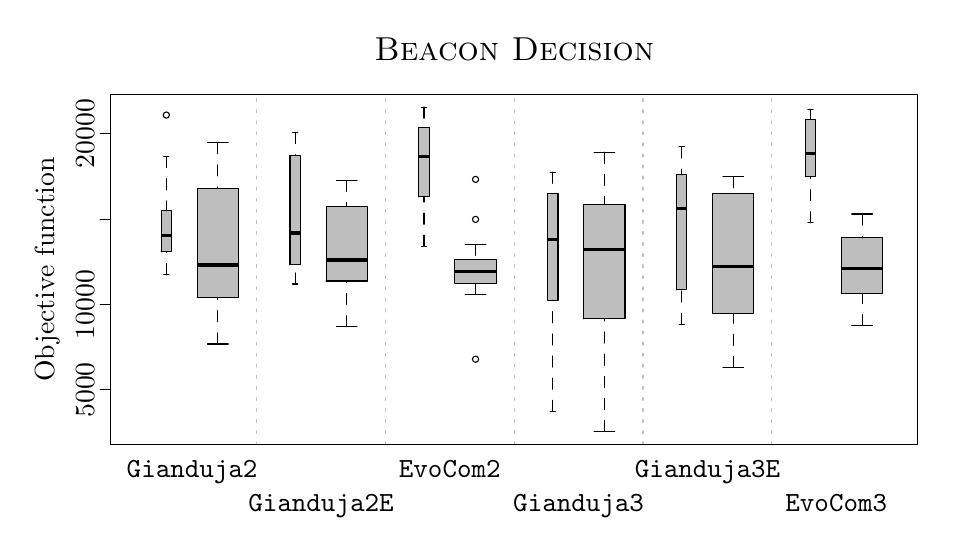
\begin{tikzpicture}[x=1pt,y=1pt]
\definecolor{fillColor}{RGB}{255,255,255}
\path[use as bounding box,fill=fillColor,fill opacity=0.00] (0,0) rectangle (325.21,180.67);
\begin{scope}
\path[clip] ( 30.00, 30.00) rectangle (321.61,156.67);
\definecolor{fillColor}{RGB}{190,190,190}

\path[fill=fillColor] ( 48.25, 99.69) --
	( 51.97, 99.69) --
	( 51.97,114.51) --
	( 48.25,114.51) --
	cycle;
\definecolor{drawColor}{RGB}{0,0,0}

\path[draw=drawColor,line width= 1.2pt,line join=round] ( 48.25,105.47) -- ( 51.97,105.47);

\path[draw=drawColor,line width= 0.4pt,dash pattern=on 4pt off 4pt ,line join=round,line cap=round] ( 50.11, 91.37) -- ( 50.11, 99.69);

\path[draw=drawColor,line width= 0.4pt,dash pattern=on 4pt off 4pt ,line join=round,line cap=round] ( 50.11,134.09) -- ( 50.11,114.51);

\path[draw=drawColor,line width= 0.4pt,line join=round,line cap=round] ( 49.18, 91.37) -- ( 51.04, 91.37);

\path[draw=drawColor,line width= 0.4pt,line join=round,line cap=round] ( 49.18,134.09) -- ( 51.04,134.09);

\path[draw=drawColor,line width= 0.4pt,line join=round,line cap=round] ( 48.25, 99.69) --
	( 51.97, 99.69) --
	( 51.97,114.51) --
	( 48.25,114.51) --
	( 48.25, 99.69);

\path[draw=drawColor,line width= 0.4pt,line join=round,line cap=round] ( 50.11,149.09) circle (  1.12);

\path[fill=fillColor] ( 61.28, 83.14) --
	( 76.18, 83.14) --
	( 76.18,122.62) --
	( 61.28,122.62) --
	cycle;

\path[draw=drawColor,line width= 1.2pt,line join=round] ( 61.28, 94.87) -- ( 76.18, 94.87);

\path[draw=drawColor,line width= 0.4pt,dash pattern=on 4pt off 4pt ,line join=round,line cap=round] ( 68.73, 66.38) -- ( 68.73, 83.14);

\path[draw=drawColor,line width= 0.4pt,dash pattern=on 4pt off 4pt ,line join=round,line cap=round] ( 68.73,139.11) -- ( 68.73,122.62);

\path[draw=drawColor,line width= 0.4pt,line join=round,line cap=round] ( 65.01, 66.38) -- ( 72.46, 66.38);

\path[draw=drawColor,line width= 0.4pt,line join=round,line cap=round] ( 65.01,139.11) -- ( 72.46,139.11);

\path[draw=drawColor,line width= 0.4pt,line join=round,line cap=round] ( 61.28, 83.14) --
	( 76.18, 83.14) --
	( 76.18,122.62) --
	( 61.28,122.62) --
	( 61.28, 83.14);

\path[fill=fillColor] ( 94.80, 95.00) --
	( 98.53, 95.00) --
	( 98.53,134.49) --
	( 94.80,134.49) --
	cycle;

\path[draw=drawColor,line width= 1.2pt,line join=round] ( 94.80,106.47) -- ( 98.53,106.47);

\path[draw=drawColor,line width= 0.4pt,dash pattern=on 4pt off 4pt ,line join=round,line cap=round] ( 96.67, 88.06) -- ( 96.67, 95.00);

\path[draw=drawColor,line width= 0.4pt,dash pattern=on 4pt off 4pt ,line join=round,line cap=round] ( 96.67,142.81) -- ( 96.67,134.49);

\path[draw=drawColor,line width= 0.4pt,line join=round,line cap=round] ( 95.73, 88.06) -- ( 97.60, 88.06);

\path[draw=drawColor,line width= 0.4pt,line join=round,line cap=round] ( 95.73,142.81) -- ( 97.60,142.81);

\path[draw=drawColor,line width= 0.4pt,line join=round,line cap=round] ( 94.80, 95.00) --
	( 98.53, 95.00) --
	( 98.53,134.49) --
	( 94.80,134.49) --
	( 94.80, 95.00);

\path[fill=fillColor] (107.84, 89.11) --
	(122.74, 89.11) --
	(122.74,115.99) --
	(107.84,115.99) --
	cycle;

\path[draw=drawColor,line width= 1.2pt,line join=round] (107.84, 96.75) -- (122.74, 96.75);

\path[draw=drawColor,line width= 0.4pt,dash pattern=on 4pt off 4pt ,line join=round,line cap=round] (115.29, 72.65) -- (115.29, 89.11);

\path[draw=drawColor,line width= 0.4pt,dash pattern=on 4pt off 4pt ,line join=round,line cap=round] (115.29,125.49) -- (115.29,115.99);

\path[draw=drawColor,line width= 0.4pt,line join=round,line cap=round] (111.56, 72.65) -- (119.01, 72.65);

\path[draw=drawColor,line width= 0.4pt,line join=round,line cap=round] (111.56,125.49) -- (119.01,125.49);

\path[draw=drawColor,line width= 0.4pt,line join=round,line cap=round] (107.84, 89.11) --
	(122.74, 89.11) --
	(122.74,115.99) --
	(107.84,115.99) --
	(107.84, 89.11);

\path[fill=fillColor] (141.36,119.54) --
	(145.08,119.54) --
	(145.08,144.73) --
	(141.36,144.73) --
	cycle;

\path[draw=drawColor,line width= 1.2pt,line join=round] (141.36,134.00) -- (145.08,134.00);

\path[draw=drawColor,line width= 0.4pt,dash pattern=on 4pt off 4pt ,line join=round,line cap=round] (143.22,101.65) -- (143.22,119.54);

\path[draw=drawColor,line width= 0.4pt,dash pattern=on 4pt off 4pt ,line join=round,line cap=round] (143.22,151.98) -- (143.22,144.73);

\path[draw=drawColor,line width= 0.4pt,line join=round,line cap=round] (142.29,101.65) -- (144.15,101.65);

\path[draw=drawColor,line width= 0.4pt,line join=round,line cap=round] (142.29,151.98) -- (144.15,151.98);

\path[draw=drawColor,line width= 0.4pt,line join=round,line cap=round] (141.36,119.54) --
	(145.08,119.54) --
	(145.08,144.73) --
	(141.36,144.73) --
	(141.36,119.54);

\path[fill=fillColor] (154.39, 88.36) --
	(169.29, 88.36) --
	(169.29, 96.85) --
	(154.39, 96.85) --
	cycle;

\path[draw=drawColor,line width= 1.2pt,line join=round] (154.39, 92.67) -- (169.29, 92.67);

\path[draw=drawColor,line width= 0.4pt,dash pattern=on 4pt off 4pt ,line join=round,line cap=round] (161.84, 84.27) -- (161.84, 88.36);

\path[draw=drawColor,line width= 0.4pt,dash pattern=on 4pt off 4pt ,line join=round,line cap=round] (161.84,102.36) -- (161.84, 96.85);

\path[draw=drawColor,line width= 0.4pt,line join=round,line cap=round] (158.12, 84.27) -- (165.57, 84.27);

\path[draw=drawColor,line width= 0.4pt,line join=round,line cap=round] (158.12,102.36) -- (165.57,102.36);

\path[draw=drawColor,line width= 0.4pt,line join=round,line cap=round] (154.39, 88.36) --
	(169.29, 88.36) --
	(169.29, 96.85) --
	(154.39, 96.85) --
	(154.39, 88.36);

\path[draw=drawColor,line width= 0.4pt,line join=round,line cap=round] (161.84,125.85) circle (  1.12);

\path[draw=drawColor,line width= 0.4pt,line join=round,line cap=round] (161.84,111.39) circle (  1.12);

\path[draw=drawColor,line width= 0.4pt,line join=round,line cap=round] (161.84, 60.87) circle (  1.12);

\path[fill=fillColor] (187.91, 82.21) --
	(191.64, 82.21) --
	(191.64,120.76) --
	(187.91,120.76) --
	cycle;

\path[draw=drawColor,line width= 1.2pt,line join=round] (187.91,104.24) -- (191.64,104.24);

\path[draw=drawColor,line width= 0.4pt,dash pattern=on 4pt off 4pt ,line join=round,line cap=round] (189.77, 42.02) -- (189.77, 82.21);

\path[draw=drawColor,line width= 0.4pt,dash pattern=on 4pt off 4pt ,line join=round,line cap=round] (189.77,128.42) -- (189.77,120.76);

\path[draw=drawColor,line width= 0.4pt,line join=round,line cap=round] (188.84, 42.02) -- (190.70, 42.02);

\path[draw=drawColor,line width= 0.4pt,line join=round,line cap=round] (188.84,128.42) -- (190.70,128.42);

\path[draw=drawColor,line width= 0.4pt,line join=round,line cap=round] (187.91, 82.21) --
	(191.64, 82.21) --
	(191.64,120.76) --
	(187.91,120.76) --
	(187.91, 82.21);

\path[fill=fillColor] (200.95, 75.45) --
	(215.84, 75.45) --
	(215.84,116.71) --
	(200.95,116.71) --
	cycle;

\path[draw=drawColor,line width= 1.2pt,line join=round] (200.95,100.52) -- (215.84,100.52);

\path[draw=drawColor,line width= 0.4pt,dash pattern=on 4pt off 4pt ,line join=round,line cap=round] (208.40, 34.69) -- (208.40, 75.45);

\path[draw=drawColor,line width= 0.4pt,dash pattern=on 4pt off 4pt ,line join=round,line cap=round] (208.40,135.66) -- (208.40,116.71);

\path[draw=drawColor,line width= 0.4pt,line join=round,line cap=round] (204.67, 34.69) -- (212.12, 34.69);

\path[draw=drawColor,line width= 0.4pt,line join=round,line cap=round] (204.67,135.66) -- (212.12,135.66);

\path[draw=drawColor,line width= 0.4pt,line join=round,line cap=round] (200.95, 75.45) --
	(215.84, 75.45) --
	(215.84,116.71) --
	(200.95,116.71) --
	(200.95, 75.45);

\path[fill=fillColor] (234.47, 85.95) --
	(238.19, 85.95) --
	(238.19,127.52) --
	(234.47,127.52) --
	cycle;

\path[draw=drawColor,line width= 1.2pt,line join=round] (234.47,115.21) -- (238.19,115.21);

\path[draw=drawColor,line width= 0.4pt,dash pattern=on 4pt off 4pt ,line join=round,line cap=round] (236.33, 73.50) -- (236.33, 85.95);

\path[draw=drawColor,line width= 0.4pt,dash pattern=on 4pt off 4pt ,line join=round,line cap=round] (236.33,137.58) -- (236.33,127.52);

\path[draw=drawColor,line width= 0.4pt,line join=round,line cap=round] (235.40, 73.50) -- (237.26, 73.50);

\path[draw=drawColor,line width= 0.4pt,line join=round,line cap=round] (235.40,137.58) -- (237.26,137.58);

\path[draw=drawColor,line width= 0.4pt,line join=round,line cap=round] (234.47, 85.95) --
	(238.19, 85.95) --
	(238.19,127.52) --
	(234.47,127.52) --
	(234.47, 85.95);

\path[fill=fillColor] (247.50, 77.42) --
	(262.40, 77.42) --
	(262.40,120.82) --
	(247.50,120.82) --
	cycle;

\path[draw=drawColor,line width= 1.2pt,line join=round] (247.50, 94.34) -- (262.40, 94.34);

\path[draw=drawColor,line width= 0.4pt,dash pattern=on 4pt off 4pt ,line join=round,line cap=round] (254.95, 57.87) -- (254.95, 77.42);

\path[draw=drawColor,line width= 0.4pt,dash pattern=on 4pt off 4pt ,line join=round,line cap=round] (254.95,126.76) -- (254.95,120.82);

\path[draw=drawColor,line width= 0.4pt,line join=round,line cap=round] (251.23, 57.87) -- (258.67, 57.87);

\path[draw=drawColor,line width= 0.4pt,line join=round,line cap=round] (251.23,126.76) -- (258.67,126.76);

\path[draw=drawColor,line width= 0.4pt,line join=round,line cap=round] (247.50, 77.42) --
	(262.40, 77.42) --
	(262.40,120.82) --
	(247.50,120.82) --
	(247.50, 77.42);

\path[fill=fillColor] (281.02,126.83) --
	(284.74,126.83) --
	(284.74,147.60) --
	(281.02,147.60) --
	cycle;

\path[draw=drawColor,line width= 1.2pt,line join=round] (281.02,135.26) -- (284.74,135.26);

\path[draw=drawColor,line width= 0.4pt,dash pattern=on 4pt off 4pt ,line join=round,line cap=round] (282.88,110.17) -- (282.88,126.83);

\path[draw=drawColor,line width= 0.4pt,dash pattern=on 4pt off 4pt ,line join=round,line cap=round] (282.88,151.15) -- (282.88,147.60);

\path[draw=drawColor,line width= 0.4pt,line join=round,line cap=round] (281.95,110.17) -- (283.81,110.17);

\path[draw=drawColor,line width= 0.4pt,line join=round,line cap=round] (281.95,151.15) -- (283.81,151.15);

\path[draw=drawColor,line width= 0.4pt,line join=round,line cap=round] (281.02,126.83) --
	(284.74,126.83) --
	(284.74,147.60) --
	(281.02,147.60) --
	(281.02,126.83);

\path[fill=fillColor] (294.05, 84.63) --
	(308.95, 84.63) --
	(308.95,104.76) --
	(294.05,104.76) --
	cycle;

\path[draw=drawColor,line width= 1.2pt,line join=round] (294.05, 93.53) -- (308.95, 93.53);

\path[draw=drawColor,line width= 0.4pt,dash pattern=on 4pt off 4pt ,line join=round,line cap=round] (301.50, 72.98) -- (301.50, 84.63);

\path[draw=drawColor,line width= 0.4pt,dash pattern=on 4pt off 4pt ,line join=round,line cap=round] (301.50,113.34) -- (301.50,104.76);

\path[draw=drawColor,line width= 0.4pt,line join=round,line cap=round] (297.78, 72.98) -- (305.23, 72.98);

\path[draw=drawColor,line width= 0.4pt,line join=round,line cap=round] (297.78,113.34) -- (305.23,113.34);

\path[draw=drawColor,line width= 0.4pt,line join=round,line cap=round] (294.05, 84.63) --
	(308.95, 84.63) --
	(308.95,104.76) --
	(294.05,104.76) --
	(294.05, 84.63);
\definecolor{drawColor}{RGB}{190,190,190}

\path[draw=drawColor,line width= 0.4pt,dash pattern=on 1pt off 3pt ,line join=round,line cap=round] ( 82.70, 30.00) -- ( 82.70,156.67);

\path[draw=drawColor,line width= 0.4pt,dash pattern=on 1pt off 3pt ,line join=round,line cap=round] (129.25, 30.00) -- (129.25,156.67);

\path[draw=drawColor,line width= 0.4pt,dash pattern=on 1pt off 3pt ,line join=round,line cap=round] (175.81, 30.00) -- (175.81,156.67);

\path[draw=drawColor,line width= 0.4pt,dash pattern=on 1pt off 3pt ,line join=round,line cap=round] (222.36, 30.00) -- (222.36,156.67);

\path[draw=drawColor,line width= 0.4pt,dash pattern=on 1pt off 3pt ,line join=round,line cap=round] (268.92, 30.00) -- (268.92,156.67);
\end{scope}
\begin{scope}
\path[clip] (  0.00,  0.00) rectangle (325.21,180.67);
\definecolor{drawColor}{RGB}{0,0,0}

\node[text=drawColor,anchor=base,inner sep=0pt, outer sep=0pt, scale=  1.00] at ( 59.42, 18.00) {\texttt{Gianduja2}};

\node[text=drawColor,anchor=base,inner sep=0pt, outer sep=0pt, scale=  1.00] at (152.53, 18.00) {\texttt{EvoCom2}};

\node[text=drawColor,anchor=base,inner sep=0pt, outer sep=0pt, scale=  1.00] at (245.64, 18.00) {\texttt{Gianduja3E}};

\node[text=drawColor,anchor=base,inner sep=0pt, outer sep=0pt, scale=  1.00] at (105.98,  6.00) {\texttt{Gianduja2E}};

\node[text=drawColor,anchor=base,inner sep=0pt, outer sep=0pt, scale=  1.00] at (199.08,  6.00) {\texttt{Gianduja3}};

\node[text=drawColor,anchor=base,inner sep=0pt, outer sep=0pt, scale=  1.00] at (292.19,  6.00) {\texttt{EvoCom3}};
\end{scope}
\begin{scope}
\path[clip] (  0.00,  0.00) rectangle (325.21,180.67);
\definecolor{drawColor}{RGB}{0,0,0}

\node[text=drawColor,anchor=base,inner sep=0pt, outer sep=0pt, scale=  1.20] at (175.81,168.67) {\textsc{Beacon Decision}};

\node[text=drawColor,rotate= 90.00,anchor=base,inner sep=0pt, outer sep=0pt, scale=  1.00] at (  9.60, 93.34) {Objective function};
\end{scope}
\begin{scope}
\path[clip] (  0.00,  0.00) rectangle (325.21,180.67);
\definecolor{drawColor}{RGB}{0,0,0}

\path[draw=drawColor,line width= 0.4pt,line join=round,line cap=round] ( 30.00, 49.80) -- ( 30.00,142.34);

\path[draw=drawColor,line width= 0.4pt,line join=round,line cap=round] ( 30.00, 49.80) -- ( 26.20, 49.80);

\path[draw=drawColor,line width= 0.4pt,line join=round,line cap=round] ( 30.00, 80.65) -- ( 26.20, 80.65);

\path[draw=drawColor,line width= 0.4pt,line join=round,line cap=round] ( 30.00,111.49) -- ( 26.20,111.49);

\path[draw=drawColor,line width= 0.4pt,line join=round,line cap=round] ( 30.00,142.34) -- ( 26.20,142.34);

\node[text=drawColor,rotate= 90.00,anchor=base,inner sep=0pt, outer sep=0pt, scale=  1.00] at ( 24.00, 49.80) {5000};

\node[text=drawColor,rotate= 90.00,anchor=base,inner sep=0pt, outer sep=0pt, scale=  1.00] at ( 24.00, 80.65) {10000};

\node[text=drawColor,rotate= 90.00,anchor=base,inner sep=0pt, outer sep=0pt, scale=  1.00] at ( 24.00,142.34) {20000};

\path[draw=drawColor,line width= 0.4pt,line join=round,line cap=round] ( 30.00, 30.00) --
	(321.61, 30.00) --
	(321.61,156.67) --
	( 30.00,156.67) --
	( 30.00, 30.00);
\end{scope}
\end{tikzpicture}
